\section{Medidas de tendencia central}

\paragraph{\'Indice y subíndices}
El símbolo $X_{j}$ representa cualquiera de los  valores $X_{1},X_{2},X_{3},...$ que puede tomar la variable discreta $X.$


El símbolo $j$ denota cualquiera de los números naturales $1,2,3,...$ y se le llama \emph{índice} (o a veces \emph{subíndice} o también \emph{contador}).




\begin{definicion}[Sumatoria]
	\begin{align}
		\sum_{j=1}^{N}X_{j}=X_{1}+...+X_{N}
	\end{align}
\end{definicion}



\begin{ejemplo}
	\begin{itemize}
		\item $\displaystyle \sum_{k=1}^{N}X_{k}Y_{k}=
		X_{1}Y_{1}+...+X_{N}Y_{N}$
		\item $\displaystyle \sum_{i=1}^{N} aX_{i}=
		aX_{1}+...+aX_{N}=a\sum_{n=1}^{N}X_{n}.$
	\end{itemize}
	
\end{ejemplo}



\begin{observacion}
	Cuando se \emph{sobrentiende} que el contador $j$ \emph{corre} sobre los números $1,2,...,N,$ escribimos $\sum X_{j}$ o simplemente $\sum X$ en lugar de $\sum_{j=1}^{N}.$
\end{observacion}


\paragraph{Linealidad}
\begin{problema}
	Si $a,b$ son constantes, demuestre que
	\begin{align}
		\sum \left( aX+bY \right)=a\sum X + b\sum Y.
	\end{align}
\end{problema}

\paragraph{Promedio}
UN \emph{promedio} es un valor representativo de un conjunto de datos que tiende a encontrarse en el centro de dicho conjunto. 

Por esta razón, también se le conoce como \emph{medidas de tendencia central.}



Se pueden definir varios tipo de promedios: 
\begin{itemize}
	\item Media aritmética;
	\item mediana;
	\item moda;
	\item media geométrica;
	\item media armónica.
\end{itemize}



\begin{observacion}
	Cada medida de tendencia central tiene ventajas y desventajas de acuerdo al tipo de datos y el propósito del uso.
\end{observacion}



\begin{definicion}[Media aritmética]
	\begin{align}
		\label{3.1}
		\bar{X} =\dfrac{X_{1}+...+X_{N}}{N} = \dfrac{\sum_{j=1}^{N}X_{j}}{N}=\dfrac{\sum X}{N}
	\end{align}
\end{definicion}



\begin{ejemplo}
	La media aritmética de $8,3,5,12,10$ es...
\end{ejemplo}



Si los números $X_{1},X_{2},...,X_{k}$ se presentan con \emph{frecuencias} $f_{1}, f_{2},...,f_{k}$ respectivamente su media aritmética es
\begin{align}
	\label{3.2}
	\bar{X}=\dfrac{f_{1}X_{1}+...+f_{k}X_{k}}{f_{1}+...+f_{k}}=\dfrac{\sum fX}{\sum f}=\dfrac{\sum fX}{N}.
\end{align}
dónde $N=\sum f$ es la \emph{suma de frecuencias} o \emph{total de casos.}


\begin{ejemplo}
	Si $5,8,6,2$ se presentan con frecuencias $3,2,4,1$ respectivamente, su media aritmética es...
\end{ejemplo}


\paragraph{Media aritmética ponderada}
Algunas veces, a los números $X_{1},...,X_{k}$ se les asignan ciertos \emph{factores de ponderación} o \emph{pesos} $w_{1},...,w_{k},$ tales que \begin{align}
	\begin{cases}
		0\% \leq w_{i}\leq 100\% \\
		\sum w_{i} = 100\%
	\end{cases}
\end{align}


\begin{definicion}[Media ponderada]
	Si $w_{1},..,w_{k}$ son \emph{pesos} tales que $0\leq w_{i}\leq 1$ y $\sum w_{i}=1,$ entonces la correspondiente media (aritmética) ponderada de los números $X_{1},...,X_{k}$ es
	\begin{align}
		\bar{X}= \dfrac{w_{1}X_{1}+...+w_{k}X_{k}}{w_{1}+...+w_{k}}=\dfrac{\sum wX}{\sum w}=\sum wX.
	\end{align}
\end{definicion}



\begin{ejemplo}
	Si en una clase, al examen final se le da el triple del valor que a los exámenes parciales y un estudiante obtiene 85 en el final y 70 y 90 en los dos exámenes parciales, obtener su media ponderada.
\end{ejemplo}



\begin{enumerate}
	\item Si $w_{i}=\frac{1}{N},$ obtenemos la media aritmética usual. 
	\item Si $w_{i}=\frac{f_{i}}{N},$ obtenemos la fórmula \eqref{3.2}.
\end{enumerate}



%%%%%%%%%%%%%%
\subsection{Datos agrupados}

Cuando los números son muy grandes, se suele utilizar un pivote $P:$ 
$$
\bar{X}=P+\dfrac{\sum f_{i}d_{i}}{N},
$$
donde $d_{i}=X_{i}-P.$

En ocasiones, utilizaremos la notación
\begin{align}
	\bar{d}=\dfrac{\sum f_{i}d_{i}}{N},
\end{align}
de manera que $\bar{d}$ es la \emph{desviación promedio} y $\bar{X}=P+\bar{d}.$



\begin{observacion}
	
	Para datos agrupados, $X_{i}$ se escoge como la marca de la $i-$ésima clase.
\end{observacion}


\paragraph{La mediana}
La mediana $\til{X}$ de un conjunto de números acomodados en un orden de magnitud (es decir, en una ordenación) es el valor central o la media de dos valores centrales.


\begin{ejemplo}
	\begin{itemize}
		\item La mediana de la lista de números $3,4,5,6,8,8,8,10$ es... 
		\item La mediana de la lista de números $5,5,7,9,11,12,15,18$ es..
	\end{itemize}
	
\end{ejemplo}



\begin{definicion}[Mediana para datos agrupados]
	\begin{align}
		\texttt{Mediana}=L+\left(
		\dfrac{ \dfrac{N}{2}-\sum_{{C<C_{M}}}f}{f_{C_{M}}}
		\right)
	\end{align}
	donde 
	\begin{itemize}
		\item $L$ es la frontera inferior de la clase mediana, es decir, de la clase que contiene la mediana;
		\item $N$ es la frecuencia total; 
		\item $\sum_{{C<C_{M}}}f$ suma de las frecuencias de todas las clases anteriores a la clase mediana; 
		\item $f_{C_{M}}$ es la frecuencia de la clase mediana.
	\end{itemize}
	
\end{definicion}


\paragraph{Moda}
La moda de una lista de números es un valor que se presenta con la mayor frecuencia $f>1$.  \emph{La moda no es necesariamente existe ni es única.}


\begin{ejemplo}
	\begin{itemize}
		\item La moda de la lista $2,2,5,7,9,9,9,10,10,11,12,18$ es...  En este caso, diremos que la lista es \emph{unimodal.}
		\item ?`Cuál es la moda de la lista $3,5,8,0,12,15,16$? 
		\item ?`Cuál es la moda de la lista $3,8,8,8,15,15,15$?  En este caso diremos que la lista es \emph{bimodal.}
	\end{itemize}
	
\end{ejemplo}



\begin{definicion}[Moda para datos agrupados]
	\begin{align}
		\texttt{Moda}=
		L + \left( \dfrac{\Del_{1}}{\Del_{1}+\Del_{2}} \right)c
	\end{align}
	donde 
	\begin{enumerate}
		\item $L:$ Frontera inferior de la clase modal, es decir, de la clase que contiene la moda.
		\item $\Del_{1}:$ Exceso de frecuencia modal sobre la frecuencia en la clase inferior inmediata. 
		\item $\Del_{2}:$ Exceso de frecuencia modal sobre la frecuencia en la clase superior inmediata. 
		\item $c:$ Amplitud del intervalo de la clase modal.
	\end{enumerate}
	
\end{definicion}


%%%%%%%%%%%%%%%%%%5
%%%%%%%%%%%%%%%%%%%%%5

\subsection{Python}

\begin{lstlisting}[language=Python]
	numpy.mean(a, axis=None, dtype=None, out=None,
	keepdims=<class numpy._globals._NoValue>)
\end{lstlisting}

Calcula  la media aritmética sobre los elementos de un arreglo. \footnote{\href{https://github.com/numpy/numpy/blob/v1.13.0/numpy/core/fromnumeric.py\#L2806-L2909}{https://github.com/numpy/numpy/blob/v1.13.0/numpy/core/fromnumeric.py\#L2806-L2909}}


[]{Ejemplos}
\begin{lstlisting}[language=Python]
	a = np.array([[1, 2], [3, 4]])
	print np.mean(a)
	#2.5
	print np.mean(a, axis=0)
	#array([ 2.,  3.])
	print np.mean(a, axis=1)
	#array([ 1.5,  3.5])
\end{lstlisting}


[]{numpy.median}
\begin{lstlisting}[language=Python]
	numpy.median(a, axis=None, out=None,
	overwrite_input=False, keepdims=False)
\end{lstlisting}

Calcula la mediana de los elementos de un arreglo de números.\footnote{\href{https://docs.scipy.org/doc/numpy/reference/generated/numpy.median.html}{https://docs.scipy.org/doc/numpy/reference/generated/numpy.median.html}}


[,]{Ejemplos}
\begin{lstlisting}[language=Python]
	import numpy as np
	
	a = np.array([[10, 7, 4], [3, 2, 1]])
	print a
	#array([[10,  7,  4],6[ 3,  2,  1]])
	print np.median(a)
	#3.5
	print np.median(a, axis=0)
	#array([ 6.5,  4.5,  2.5])
	print np.median(a, axis=1)
	#array([ 7.,  2.])
	
	m = np.median(a, axis=0)
	out = np.zeros_like(m)
	print np.median(a, axis=0, out=m)
	#array([ 6.5,  4.5,  2.5])
	print m
	#array([ 6.5,  4.5,  2.5])
	b = a.copy()
	print np.median(b, axis=1, overwrite_input=True)
	#array([ 7.,  2.])
	
	assert not np.all(a==b)
	b = a.copy()
	print np.median(b, axis=None, overwrite_input=True)
	#3.5
	assert not np.all(a==b)
\end{lstlisting}


\paragraph{\text{SciPy}}
SciPy es una biblioteca open source de herramientas y algoritmos matemáticos para Python...

SciPy contiene módulos para optimización, álgebra lineal, integración, interpolación, funciones especiales, FFT, procesamiento de señales y de imagen, resolución de ODEs y otras tareas para la ciencia e ingeniería. Está dirigida al mismo tipo de usuarios que los de aplicaciones como MATLAB, GNU Octave, y Scilab.\footnote{\href{https://es.wikipedia.org/wiki/SciPy}{https://es.wikipedia.org/wiki/SciPy}}

[, ]{Moda}
\begin{lstlisting}[language=Python]
	import numpy as np
	from scipy import stats
	
	a = np.array([3,5,6,5,6,5,6,6,3,1,5])
	print stats.mode(a)
	# ModeResult(mode=array([5]), count=array([4]))
\end{lstlisting}

\begin{lstlisting}[language=Python]
	b = np.array([[6, 8, 0, 0],
	[3, 3, 0, 3],
	[8, 1, 8, 5],
	[5, 3, 0, 5],
	[4, 7, 5, 3]])
	
	print stats.mode(b)
	# ModeResult(mode=array([[3, 3, 0, 3]]),
	count=array([[1, 2, 3, 2]]))
\end{lstlisting}

\begin{lstlisting}[language=Python]
	print stats.mode(b, axis=1)
	# ModeResult(mode=array([[0],[3],[8],[5],[3]]),
	#           count=array([[2],[3],[2],[2],[1]]))
	
	print stats.mode(b, axis=None)
	# ModeResult(mode=array([3]), count=array([5]))
\end{lstlisting}

%
\begin{problema} \label{problema:3.1}
	Escribir los términos de cada una de las siguientes sumas:
	\begin{enumerate}
		\item $\displaystyle\sum_{j=0}^{6}X_{j}=$ 
		\item $\displaystyle\sum_{k=1}^{4}\left( Y_{k}-3 \right)^{2}=$ 
		\item $\displaystyle\sum_{k=1}^{N}a=$ 
		\item $\displaystyle\sum_{n=2}^{5}{f_{n}}X_{n}= $ 
		\item $\displaystyle\sum_{m=0}^{3}\left( X_{m}-a \right)=$
	\end{enumerate}
	%
	%
\end{problema}
%


\begin{problema}
	\label{problema:3.10}
	De 100 números, 20 fueron 4, 40 fueron 5, 30 fueron 6 y los restantes fueron 7. Encuentre su media aritmética.
\end{problema}




\begin{problema}
	\label{problema:3.13}
	Los pesos medio de cuatro grupos de estudiantes que constan de 15, 20, 10 y 18 individuos son 162, 148, 153 y 140 libras, respectivamente. Encuentre el peso medio de todos los estudiantes.
\end{problema}



%

\begin{problema}
	\label{problema:3.15}
	
	Usando la distribución de frecuencias de las estaturas que se presenta en la siguiente tabla, hallar la estatura media de 100 estudiantes de cierta universidad.
	\begin{figure}
		%%%%%%%%%%%%%%%%%%%%%%%%%%%%%%%%%%%%%%%%%%%%%%%%%%%%%%%%%%%%%%%%%%%%%%%%%%%%%%%%%%%%%%%
		%%% You will need to add \usepackage{wrapfig} to your preamble to use textwrapping %%%
		%%%%%%%%%%%%%%%%%%%%%%%%%%%%%%%%%%%%%%%%%%%%%%%%%%%%%%%%%%%%%%%%%%%%%%%%%%%%%%%%%%%%%%%
		\centering
		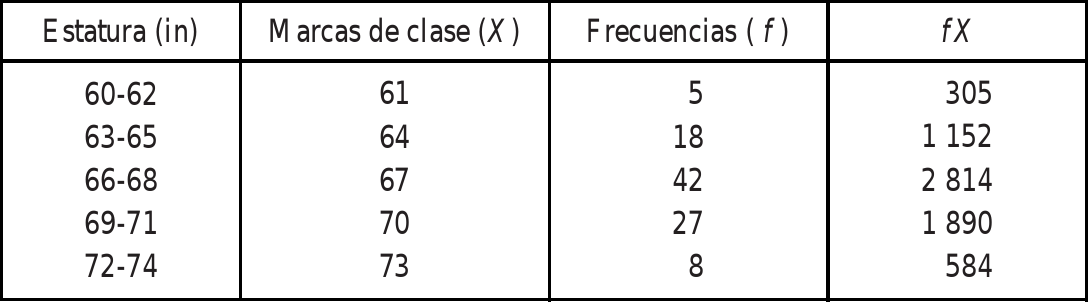
\includegraphics[width=10cm,keepaspectratio=true]{./images/tab0301.png}
		% tab0301.png: 0x0 pixel, 300dpi, 0.00x0.00 cm, bb=
		\label{tab:0301}
	\end{figure}
\end{problema}




\begin{problema}
	\label{problema:3.18}
	Si las desviaciones de $N$ números $X_{1},..,X_{N}$ respecto a un \emph{pivote} $P$ están dada por $d_{i}=X_{i}-P, \; i=1,...,N$ respectivamente, demostrar que
	\begin{align}
		\bar{X}=P+\dfrac{\sum d}{N}.
	\end{align}
\end{problema}



\begin{problema}
	\label{problema:3.16}
	Demostrar que la suma de las desviaciones $d_{1},d_{2},...,d_{N}$ de $X_{1},X_{2},...,X_{N}$ usando como pivote su media $\bar{X}$ es igual a cero.
\end{problema}



\begin{problema}
	\label{problema:3.17}
	Si $Z_{i}=X_{i}+Y_{i}, \; i=1,2,...,N,$ demostrar que $\bar{Z}=\bar{X}+\bar{Y}.$
\end{problema}




\begin{problema}
	\label{problema:3.19}
	Halle la media aritmética de los números 5,8,11,9,12,6,14 y 10 eligiendo como \emph{pivote} a) $P=9$ y b) $P=20.$
\end{problema}




\begin{problema}
	\label{problema:3.20}
	Utilice la marca de la clase media como pivote, para calcular la estatura de los estudiantes en la tabla \ref{tab:0301}.
\end{problema}



\begin{problema}
	\label{problema:3.28}
	Encontrar el peso mediano a partir de la siguiente tabla
	\begin{figure}[ht]
		\centering
		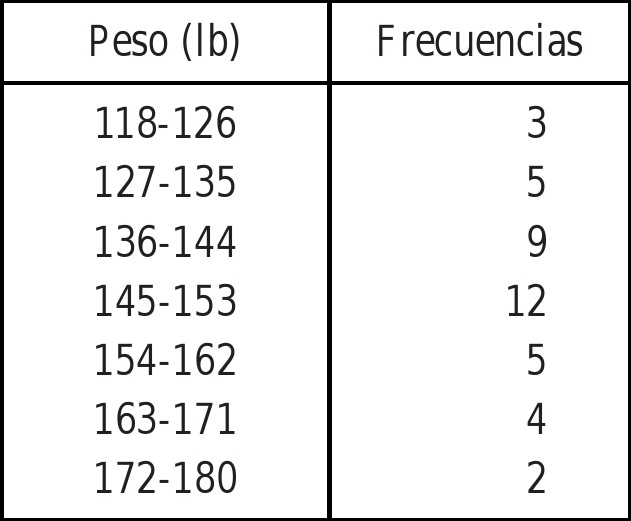
\includegraphics[height=5cm,keepaspectratio=true]{./images/tab0307.png}
		% tab0307.png: 0x0 pixel, 300dpi, 0.00x0.00 cm, bb=
		\label{tab:0307}
	\end{figure}
	
\end{problema}


